\begin{wrapfigure}[14]{r}{0.4\textwidth}
       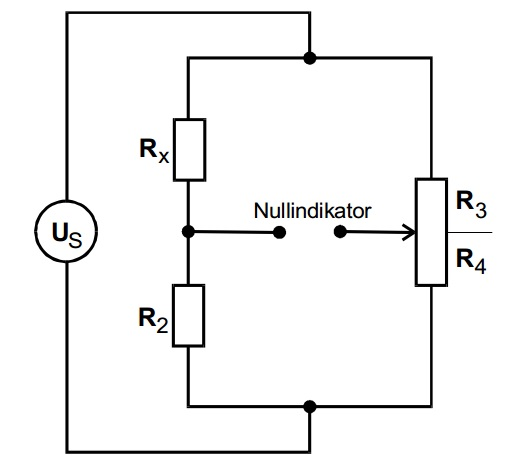
\includegraphics[scale=0.5]{Grafiken/Wheat}
       \caption{Wheatstonesche Brückenschaltung \cite{V302}}
       \label{fig:Wheat}
\end{wrapfigure}
\subsection{Aufbau}
Im Experiment werden fünf Brückenschaltungen aufgebaut und vermessen. \\
Die erste Brücke, bei der es einen realen Widerstand zu messen gilt, ist die Wheatstone'sche Brücke. Sie besteht im Wesentlichen aus einem bekannten und einem unbekannten Widerstand, Spannungsversorgung und zum Ablesen der Oszillograph. Das Verhältnis von $R_3/R_4$ wird in der Schaltung mit einem Potentiometer realisiert.\\
Sowohl die Kapazitäts-, als auch die Induktivitätsmessbrücke haben einen analogen Aufbau, hier sind lediglich zu $R_x$ und $R_2$ Kondensatoren bzw. Spulen zwischen geschaltet, um einen komplexen Widerstand in die Schaltung einzubauen, dabei dienen $R_x$ und $R_2$ als Stellglied, sprich stellvertretend für die dielektrische Verlustwärme, die z.B. durch Wärme entsteht.
Bei der Maxwell-Brücke wird wie bei der Induktivitätsmessbrücke eine Spule $L_x$ mit einem Stellglied und $R_2$ in Reihe geschaltet, parallel dazu ist - entgegen der Anleitung - wieder das Potentiometer geschaltet, dieses mal ist es allerdings zusätzlich $R_4$ mit einem bekannten Kondensator $C_4$ parallel geschaltet.\\
Nun folgt noch die Wien-Robinson-Brücke, sie soll keine Abgleichelemente haben.
Der Aufbau ähnelt dem der Maxwellbrücke in gewissem Maße: $L_x$ und $R_x$ werden hier durch den doppelten Widerstand $R_2$ ersetzt und nun $R'$ genannt, zusätzlich wird der verstellbare Widerstand $R_3$ durch einen Kondensator mit einem festen Widerstand $R$ ($\neq R'$) ersetzt, außerdem ist $R_4$ natürlich nun auch nicht mehr verstellbar, da nun nur noch die Frequenz geändert wird.
Die Wien-Robinson-Brücke fungiert als Frequenzfilter. \\

\subsection{eigentliche Durchführung}
Zu erst wird die Wheatstone'sche Brücke mit 3 verschiedenen $R_2$ für eine Unbekannte $R_x$ mit Hilfe des Potentiometers ausgemessen, dabei wird ein Minimum für die dargestellte Spannung am Oszillographen gesucht. \\
Das wird dies analog für die Kapazitätsmessbrücke und für die Induktivitätsmessbrücke durchgeführt, allerdings nur für zwei anstatt drei bekannte Spulen und für die Maxwell-Brücke anstelle der dritten Spule nur ein Mal. \\
Zuletzt werden noch für die Wien-Robinson-Brücke die Peak-to-Peak-Spannung für die Frequenzen von 20 bis 30.000 Hertz abgelesen.

\begin{figure}[h]
\centering
\subfloat[Kapazitätsmessbrücke \label{pic:Kapazitaet}]{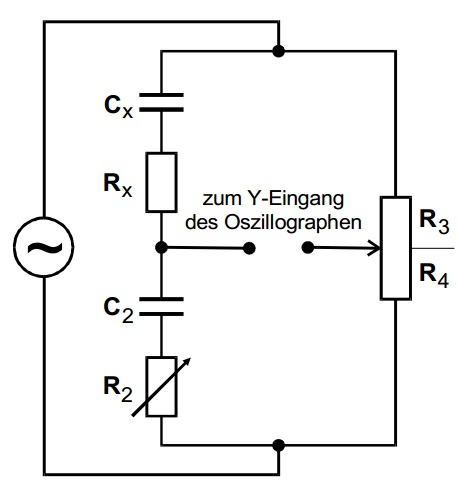
\includegraphics[scale=0.4]{Grafiken/Kapazitaet}}
\hspace{2.5cm}
\subfloat[Induktivitätsmessbrücke \label{pic:Induktivitaet}]{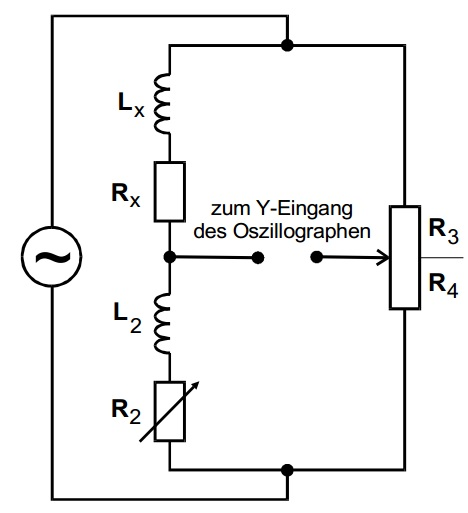
\includegraphics[scale=0.4]{Grafiken/Induktivitaet}}
\hfill
\caption{Kapazitätsmessbrücke und Induktivitätsmessbrücke \cite{V302}}
\label{Gesamtbild1}
\end{figure}
\begin{figure}[h]
\centering
\subfloat[Maxwell-Brücke \label{pic:Maxwell}]{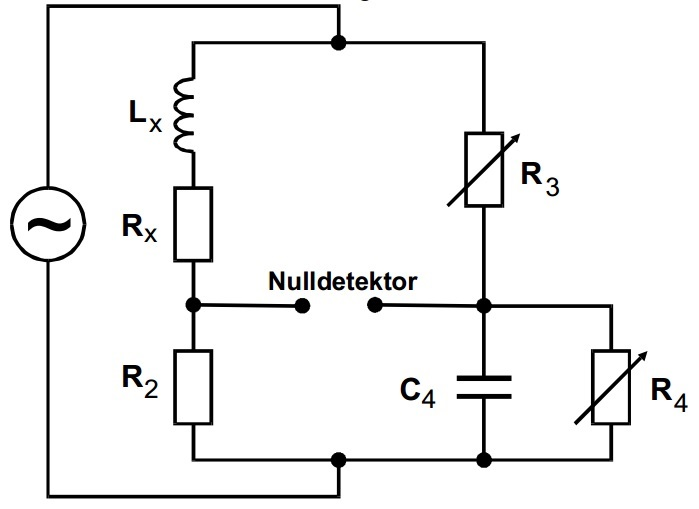
\includegraphics[scale=0.3]{Grafiken/Maxwell}}
\hspace{1.4cm}
\subfloat[Wien-Robinson-Brücke \label{pic:WienRobinson}]{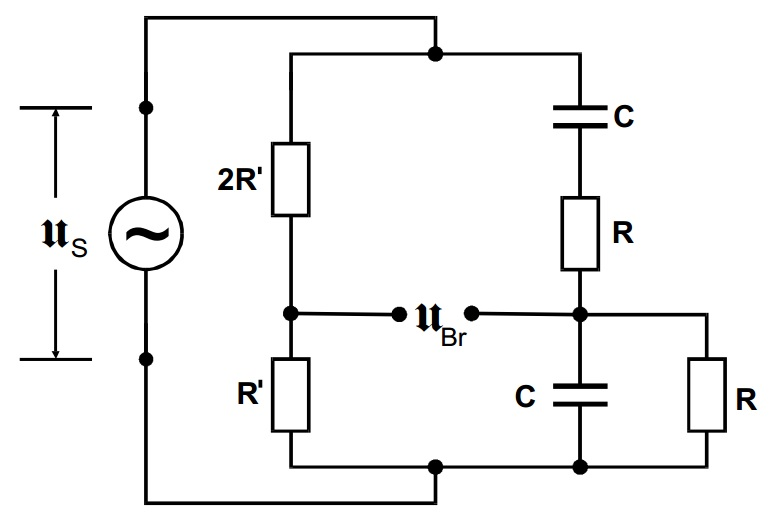
\includegraphics[scale=0.3]{Grafiken/WienRobinson.jpg}}
\hfill
\caption{Maxwell-Brücke und Wien-Robinson-Brücke \cite{V302}}
\label{Gesamtbild2}
\end{figure}
